\documentclass{article}
\usepackage{graphicx} % Required for inserting images
\usepackage{listings}
\usepackage{xcolor}
\usepackage{float}
\usepackage[backend=biber,style=apa]{biblatex}
\addbibresource{referencias.bib}
\title{Implementación de algoritmos de generación procedural para la creación de niveles de Geometry Dash}
\author{
    \begin{minipage}{0.5\textwidth}
        \centering
        \small
        Simon Gallardo \\
        \texttt{sgallardo23@alumnos.utalca.cl}
    \end{minipage}%
    \begin{minipage}{0.5\textwidth}
        \centering
        \small
        Rodrigo Díaz \\
        \texttt{rdiaz23@alumnos.utalca.cl}
    \end{minipage}
}
\date{Junio 2025}

\begin{document}

\maketitle
\section{Abstract}
La generación procedural de contenido puede ser aplicada en muchos contextos, entre ellos los videojuegos, se hizo un experimento con el juego geomety dash con el objetivo de saber si es realmente viable crear niveles jugables con este metodo. Para la aplicación del estudio se usó el algoritmo de las cadenas de Markov el cual permite crear contenido en base fragmentos basados en parte de ese contenido que se tiene certeza de que funciona. Se crearon 3 niveles en 3 dificultades diferentes dando como resultado que si es posible crear niveles para el juego mediante este metodo y puede ser escalable para así hacer niveles incluso más fieles a lo que se vería en el juego oficial.

\section{Introducción}
Geometry dash es un juego de plataformas que salió el año 2013 por RobTop games en el que el objetivo principal es terminal niveles sorteando obstaculos como pinchos, bloques, cierras, etc. Este juego se diferencia del resto de su genero ya que permite una gran cantidad de vehiculos los cuales se controlan de distintas formas lo que lo hace bastante retador aveces. Debido a como se estructuran estas etapas creemos que este juego puede ser victima del estudio para generación procedural de contenido mediante el algoritmo de cadenas de Markov ya que permite crear en base a patrones ya establecidos, Como explica \cite{barriola2016pagerank} las cadenas de Markov se basan en matrices de trancisión donde cada fila contiene las probabilidadesde pasar de un estado a otro dando como resultado comportamientos secuenciales, donde la sección A puede ir a B y luego a C, por ende A también puede ir a C directamente \cite{gagniuc2017markov}. Dado ese comportamiento creemos que el resultado para generar niveles de geometry dash puede ser interesante.



\section{Videojuegos y Cadenas de Markov (estado del arte)}
Las cadenas de Markov son un modelo matematico e implementable como algoritmo que describe sistemas de transición entre estados con cierta probabilidad. Este se usa para distintos propositos relacionados con la predicción de comportamientos, probabilidades, y en los que nos enfocaremos en esta investigación, la generación de contido proceduralmente. En videojuegos particularmente se han usado para la predicción de movimiento en juegos del genero MOBA \cite{zhang2019moba}.Y el caso que nos incumbe, la generación de niveles y mapas, bien funcionales y especialmente probados y utilizados en videojuegos 2D de plataformas como Super Mario Bros o Kid Icarus\cite{snodgrass2017markov}.

\section{Metodologia}
Para poner a prueba este experimento lo que haremos será crear distintas planillas o slices que representarán distintos elementos del juego. (ya que se trata de motivos de estudio lo más complejo que habrá será el cambio de cubo a nave y viceversa). Se crearán 3 maquetas distintas basadas en los slices que se usaron para "entrenar" al algoritmo y posteriormente las pasaremos al juego mediante su editor de niveles y evaluaremos los siguientes criterios:
\begin{itemize}
    \item Completabilidad
    \item Variedad y jugabilidad
\end{itemize}
\subsection{Parametros}
Los parametros que considera el algoritmo son principalmente 2 los cuales son la dificultad del nivel y la duración de este. La dificultad será medida en 3 posibles variantes:
\begin{itemize}
    \item Facil
    \item Medio
    \item Dificil
\end{itemize}
y la forma en la que afectará a la creación del nivel es que dependiendo de la dificultad el algoritmo premia o penaliza ciertos elementos en la creación del nivel como los pinchos por ejemplo, en dificultad facil se trataran de evitar, mierntras que en dificil se premia la aparición de estos.
La duración contempla cuantos slices considera al momento de crear el nivel, por lo que mientras mayor sea el numero, más slices considerará dando como resultado un nivel largo o corto en función de ese parametro. Por ultimo otro parametro que afecta a la creación de un nivel es la matriz de adyacencia que maneja las probabilidades de aparición de los slices en base a desabilidad, dificultad y trancisiones lógicas.
\subsection{Simbologia}
\begin{itemize}
    \item \texttt{*} = pincho
    \item  \texttt{\#} = Bloque
    \item \texttt{C} = Portal de cubo
    \item \texttt{S} = Portal de nave
    \item  \texttt{\_} = suelo
\end{itemize}
como ejemplo un nivel podria verse de la siguente manera:
\begin{lstlisting}
#### C ####
|      *  #
|         #
#### S ####
\end{lstlisting}






\section{Analisis de resultado}
\paragraph{1 Facil}
En las figuras de la 1 a la 4 podemos ver el nivel generado para la dificultad facil, podemos observar la completa aucencia de pinchos y predominación de bloques por lo que en teoria el algoritmo funciona como esperabamos para esta dificultad, jugablemente el nivel es competable, pero peca de ser bastante repetitivo al haber muchas veces repetido el patrón de la nave, esto tambien da como resultado que en ocaciones terminemos jugando con la nave secciones que estaban pensadas para el cubo, pero nunca se generó algo que nos hiciera jugar con el cubo una sección de nave, por lo que el algoritmo funciona bien haciendo uso de las probabilidades de uso para las slices priorizando secciones jugables.
\paragraph{2 Medio}
En las figuras de la 5 a la 9 encontramos el nivel generado en medio, el resultado es similar al primero con la diferencia que ahora hay secciones que contiene pinchos, pero tiene un salto demasiado preciso lo que permite concluir que por la forma en la que estan hechos los slices con los que se entrenó la IA existe una posibilidad de que los niveles de otras dificultades sean más dificil que esa propia dificultad
\paragraph{3 Dificil}
Finalmente en la dificultad más alta podemos ver que los pinchos salen con más frecuencia que las otras 2 y en 2 ocaciones hay una seccion con la nave bastante estrecha por lo que se cumple con la dificultad.

\subsection{Niveles generados}
Facil: 
\begin{figure}[H]
    \centering
    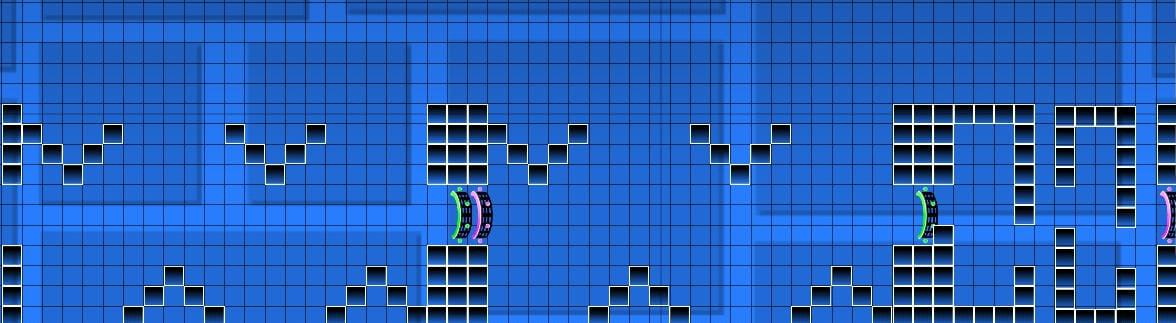
\includegraphics[width=0.8\textwidth]{Niveles/Facil/E1.jpg}
    \caption{Nivel facil parte 1.}
    \label{facil_1}
\end{figure}
\begin{figure}[H]
    \centering
    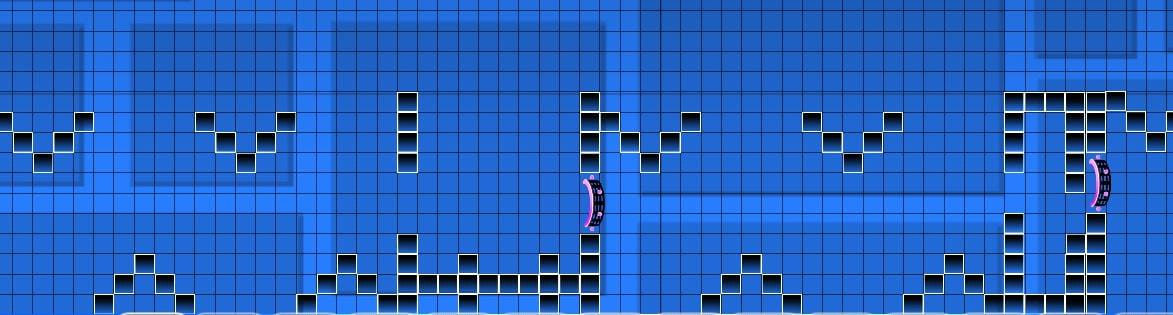
\includegraphics[width=0.8\textwidth]{Niveles/Facil/E2.jpg}
    \caption{Nivel facil parte 2.}
    \label{facil_2}
\end{figure}
\begin{figure}[H]
    \centering
    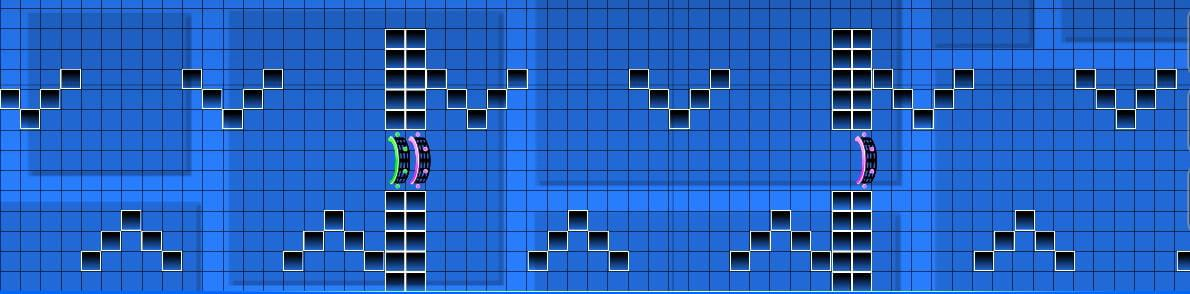
\includegraphics[width=0.8\textwidth]{Niveles/Facil/E3.jpg}
    \caption{Nivel facil parte 3.}
    \label{facil_3}
\end{figure}
\begin{figure}[H]
    \centering
    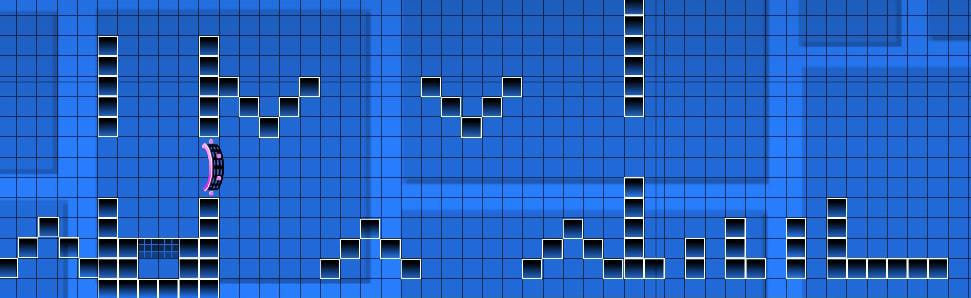
\includegraphics[width=0.8\textwidth]{Niveles/Facil/E4.jpg}
    \caption{Nivel facil parte 4.}
    \label{facil_4}
\end{figure}
Medio:
\begin{figure}[H]
    \centering
    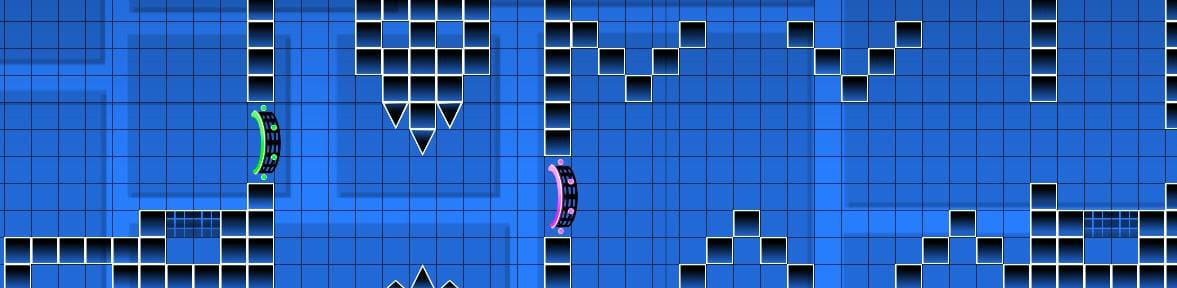
\includegraphics[width=0.8\textwidth]{Niveles/Medio/M1.jpg}
    \caption{Nivel medio parte 1.}
    \label{medio_1}
\end{figure}
\begin{figure}[H]
    \centering
    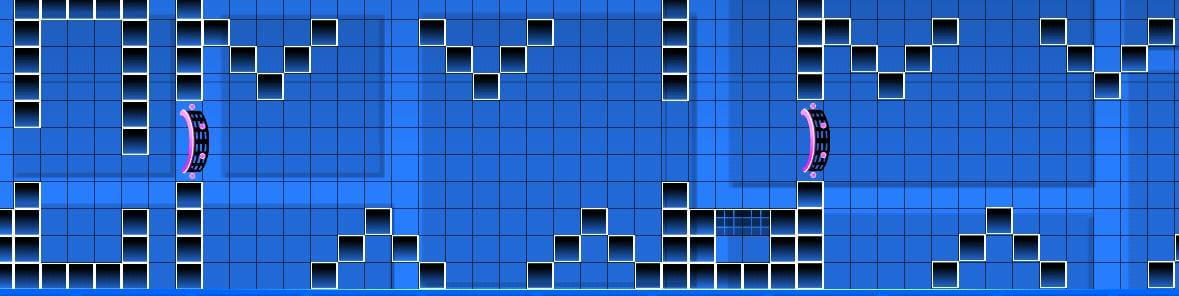
\includegraphics[width=0.8\textwidth]{Niveles/Medio/M2.jpg}
    \caption{Nivel medio parte 2.}
    \label{medio_2}
\end{figure}
\begin{figure}[H]
    \centering
    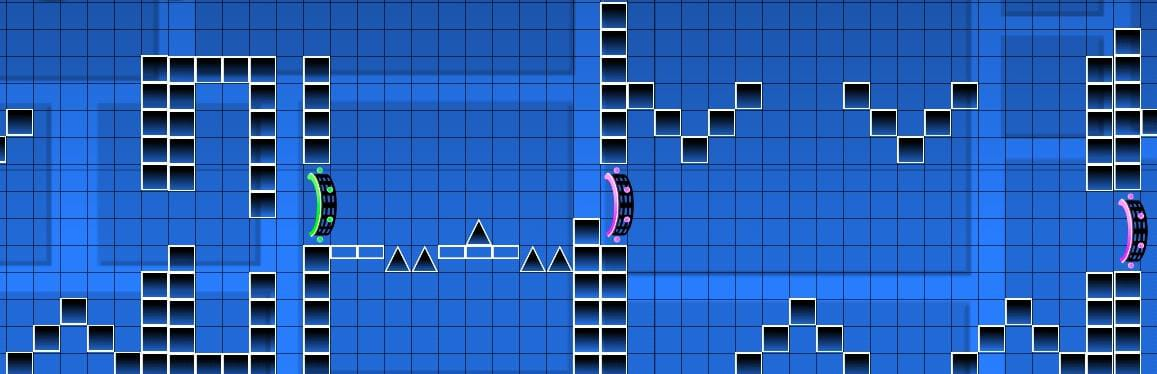
\includegraphics[width=0.8\textwidth]{Niveles/Medio/M3.jpg}
    \caption{Nivel medio parte 3.}
    \label{medio_3}
\end{figure}
\begin{figure}[H]
    \centering
    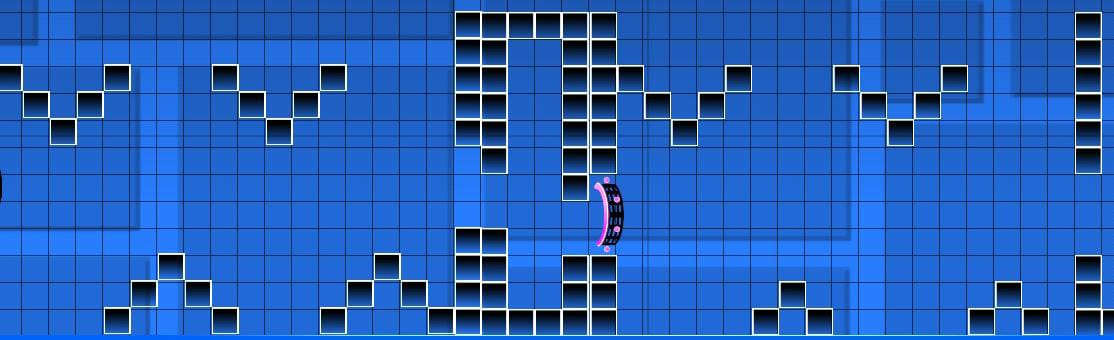
\includegraphics[width=0.8\textwidth]{Niveles/Medio/M4.jpg}
    \caption{Nivel medio parte 4.}
    \label{medio_4}
\end{figure}
\begin{figure}[H]
    \centering
    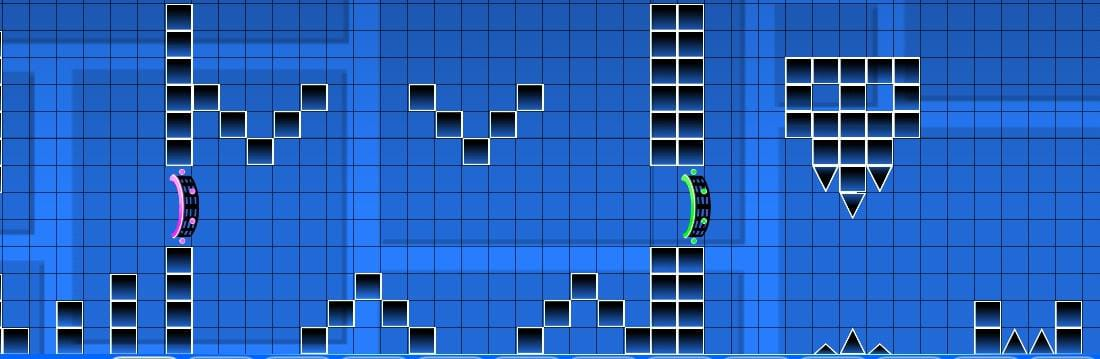
\includegraphics[width=0.8\textwidth]{Niveles/Medio/M5.jpg}
    \caption{Nivel medio parte 5.}
    \label{medio_5}
\end{figure}
Dificil:
\begin{figure}[H]
    \centering
    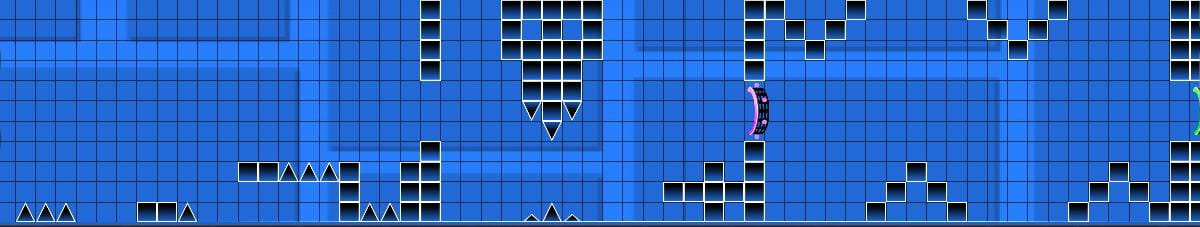
\includegraphics[width=0.8\textwidth]{Niveles/Dificil/d1.jpg}
    \caption{Nivel dificil parte 1.}
    \label{dificil_1}
\end{figure}
\begin{figure}[H]
    \centering
    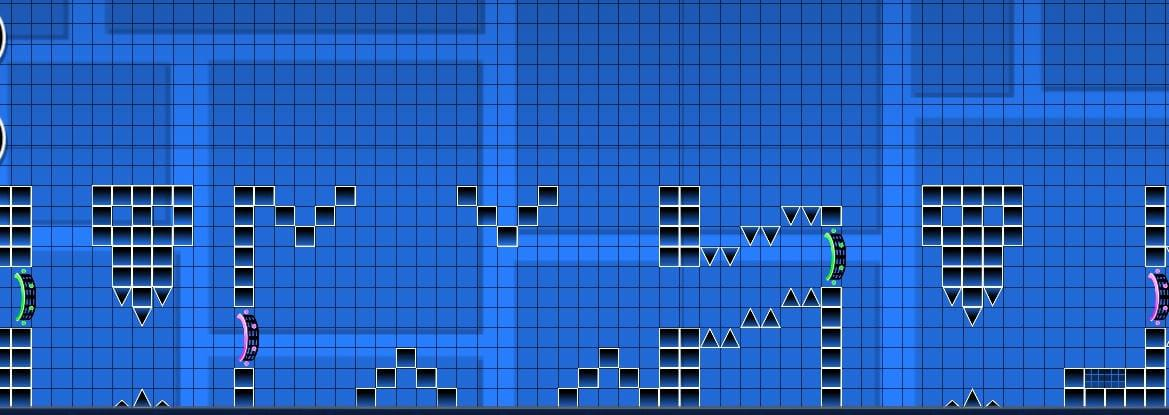
\includegraphics[width=0.8\textwidth]{Niveles/Dificil/d2.jpg}
    \caption{Nivel dificil parte 2.}
    \label{dificil_2}
\end{figure}
\begin{figure}[H]
    \centering
    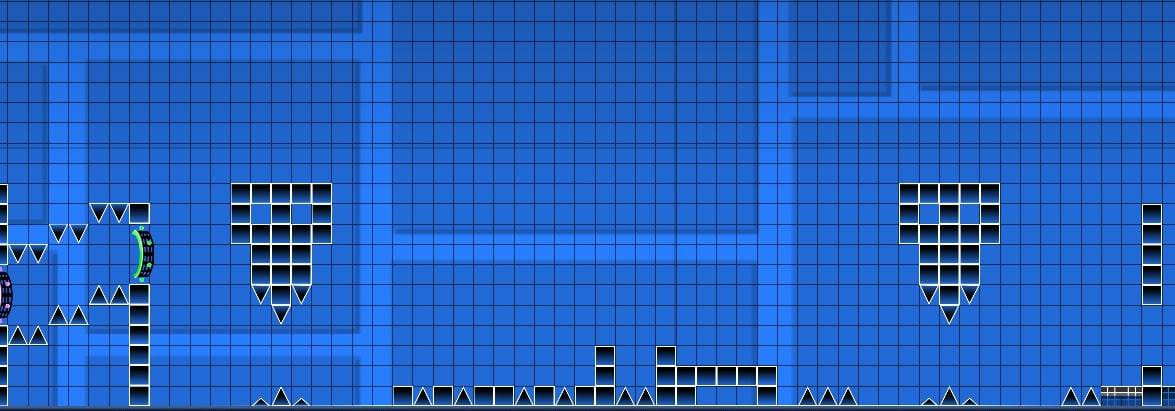
\includegraphics[width=0.8\textwidth]{Niveles/Dificil/d3.jpg}
    \caption{Nivel dificil parte 3.}
    \label{dificil_3}
\end{figure}
\subsection{Notas*}
\begin{itemize}
    \item Las maquetas generadas por el algoritmo serán adjuntadas en un archivo txt
    \item ID niveles
    \begin{itemize}
        \item Facil: 121681697
        \item Medio: 121681692
        \item Dificil: 1216811701
    \end{itemize}
\end{itemize}


\section{Discusión}
Llegados a este punto considerando como funciono el algoritmo nos queda hacernos la pregunta ¿funcionó como esperabamos? la respuesta es que si, ya que como vimos el algoritmo fue capaz de generar niveles completamente jugables, sumado a eso se podrian cambiar ciertos parametros como hacer cada slice más detallado en lugar de hacer secciones completas y se podria aumentar aún más la calidad del nivel generado, del mismo modo podriamos considerar otros vehiculos como el Ufo o la Wave e incluso agregar portales como los gravitatorios o las orbes para hacer niveles aún más completo. Como podriamos hacer esto, modificando la matriz de adyacencia para que contemple tambien las nuevas funciones y considere probabilidades basadas en estos nuevos parametros, asi mismo podriamos incluir más dificultades como la demon que podria priorizar espacios estrechos o de incluirlos, portales gravitatorios mezclados con algún vehiculo como la nave.

\section{Conclusiones}
En base a estos resultados podemos ver que es posible generar niveles funcionales para geometry dash basado en el algoritmo de cadenas de markov y que lo repetitivo de los niveles generados se debe a la falta de contenido con el que el algoritmo fue entrenado, pero si hicieramos que cada slice fuera más detallado en lugar de ser secciones completas podriamos tener niveles que se asemejen más a los diseñados por su creador, tambien se podria entrenar al algoritmo para que cambie el como considera las probabilidades y evitar casos como el del salto preciso de la dificultad media, pero sin duda es una herramienta funcional, por lo mismo mejorarla para que considere otras funciones del juego como vehiculos, portales, nuevas dificultades o incluso cambios de velocidad podrian hacer que se generacen niveles mucho más interesantes de los presentados.
\printbibliography
\end{document}
